\begin{figure}%[t]
  \centering
  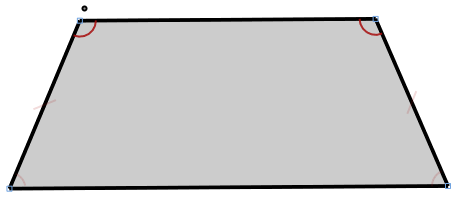
\includegraphics[width=0.7\linewidth]{img/same-angle-symmetry.png}
  \caption[Same Angle]{The Same Angle constraint can be used to create
    symmetric shapes. Here the top angles are the same (about 135
    degrees), and the lower corners are also constrained (about 45
    degrees). Because the sides are constrained to be the same length,
    the top and bottom line segments are parallel.}
  \label{fig:same-angle}
\end{figure}
